% ---
% Capitulo de revisão de literatura
% ---
\chapter{Revisão da Literatura}
\label{revisao-literatura}

A revisão de literatura é um processo de pesquisa, análise e descrição. A investigação sobre o tema tem como alvo não só os livros, mas também artigos de periódico, de jornais, relatórios governamentais, teses, dissertações, entre outros materiais \cite{revisao}.

%Todos trabalhos devem possuir a revisão de literatura onde são abordados os estudos feitos com base da literatura (livros, artigos acadêmicos, publicações em periódicos), todos elementos devem ser referenciados por citações.

%Não são abordados aqui itens técnicos que normalmente são vistos em disciplinas anteriores do curso (UML, banco de dados, metodologias de gerenciamento de projeto etc...)
\section{Solidão na pandemia}
O Instituto Ipsos realizou, entre 23 de dezembro de 2020 e 08 de janeiro de 2021, o levantamento \textit{“Perceptions of the Impact of Covid-19”} composto por perguntas sobre o bem-estar mental de 23.004 pessoas - desses, mil participantes eram brasileiros -, de 28 países, com idade em torno de 16 e 74 anos. De acordo com o levantamento, na questão \textit{“How often do you feel lonely?”} (Com que frequência você se sente solitário?) o Brasil teve o maior índice, 50\%, sendo que a média global foi de 33\%. Já no segundo semestre, 52\% dos brasileiros apontaram o aumento da solidão, novamente acima da média de todos os países, que foi de 41\% \cite{solidaoIPSOS}.

Como forma de suprir essa solidão, os brasileiros foram em busca de companheiros por meio da adoção de animais domésticos. Nesse período, a busca de animais para adoção teve aumento em 400\% - dado divulgado pela \ac {UIPA}. É importante ressaltar que não se pode agir por impulso na adoção, visto que após a pandemia as coisas irão voltar ao normal \cite{usp}. 

Não só os números de adoção aumentaram, como também os de abandono frente ao pior momento da pandemia. Dessa forma, o abandono ou até mesmo a falta dos cuidados recebidos por defensores e admiradores de animais que tiveram que mudar a rotina devido ao isolamento social, causaram e causam sofrimento para os animais \cite[p. 34-35]{isolamento-animais}. Deve ser lembrado que cães e gatos, como outros animais, são seres sencientes, ou seja, seres capazes de experienciar sentimentos, inclusive a solidão \cite{seres}.

\section{Relação entre humanos e animais}

A relação entre seres humanos e animais se tornou mais pessoal a cerca de 12.000 anos atrás no sudoeste da Ásia, na China e na América do Norte quando os humanos começaram a domesticar os lobos asiáticos. Restos mortais de ambas as espécies encontradas lado a lado dão suporte a essa teoria. O biólogo e fisiologista americano Jared Diamond afirma que "Esse processo teve profunda influência no desenvolvimento da economia e da estratificação social dos primeiros grupos humanos, levando ao surgimento das primeiras sociedades estáveis", com "esse processo" ele faz referência a domesticação \cite{lobos}.

Essa relação tornou-se tão importante que hoje em dia acredita-se que ser tutor de um animal traz benefícios a saúde. A endocrinologista do Monte Sinai, Dra. Caroline Kramer, líder de uma análise chamada "A revisão dos benefícios para a saúde do melhor amigo do homem", afirma que "Nossa análise descobriu que ter um cachorro, na verdade protege contra a morte de qualquer causa". Essa análise envolveu cerca de 4 milhões de pessoas nos Estados Unidos, Canadá, Escandinávia, Nova Zelândia, Austrália e Reino Unido. Quando focamos nas pessoas que já tiveram um ataque cardíaco ou derrame, é possível observar que o benefício de ter um pet é ainda maior, "Elas tem um risco 31\% menor de morrer de doenças cardiovasculares", afirma Kramer \cite{cardio}.

Mesmo com esses dados e mais estudos sendo desenvolvidos no campo de objetivo semelhante, o  Dr. Glenn Levine, presidente do grupo de redação do \ac{AHA} afirma que "o objetivo principal de adotar, resgatar ou comprar um animal de estimação não deve ser reduzir o risco cardiovascular", pois, a posse de um animal de estimação é um compromisso de cuidado que vem com certos custos e responsabilidades financeiras. Um animal deve ser desejado para além dos benefícios que supostamente pode trazer \cite{aha}.

Quando saímos do campo físico e focamos nos benefícios psicológicos de ter um animal como companhia podemos citar tópicos como: aumento na atividade física, companhia diária, redução da ansiedade, aumento da auto-estima (animais são ótimos ouvintes, oferecem amor incondicional e não criticam), podem ajudar seus tutores a fazerem novos amigos (por exemplo, em grupos online voltados para cuidados animais e pet shops) e eles também auxiliam na saúde mental ao criarem uma rotina ao redor dos cuidados que o pet necessita \cite{mental}.

A solidão pode ser tão mortal quanto fumar 15 cigarros por dia, prejudicando seriamente o emocional humano, tornando-se uma séria ameaça à saúde pública. A \ac{HABRI}, em conjunto com a Mars Petcare, fez uma extensa pesquisa sobre como enfrentar a crise de solidão em nossa sociedade com o poder do vínculo humano-animal. Steven Feldman, Diretor Executivo da \ac{HABRI}, afirma que “Há evidências crescentes de que os animais de estimação podem desempenhar um papel importante em ajudar as pessoas a se sentirem menos solitárias e mais conectadas socialmente”. Em entrevista com 2.000 pessoas nos Estados Unidos, foi descoberto que 85\% dos entrevistados acreditam que a interação com animais pode ajudar a reduzir a solidão. A simples existência destes animais vem nos ajudando a enfrentar períodos difíceis \cite{mentalpets}.

\section{Adoção consciente}
A adoção é um ato de bondade e uma atitude que transforma a vida tanto do animal quanto a de quem adota. A partir do momento da decisão de trazer um animal de estimação para casa, a pessoa deve estar ciente de todas as responsabilidades geradas por esse ato. Por isso, a busca pela adoção consciente é tão almejada pelas instituições de defesa dos animais fazendo com que as novas famílias possam garantir o bem-estar do pet. 

Em 2019, o Instituto de Instituto Brasileiro de Geografia e Estatística (IBGE) registrou que em aproximadamente 46\% das casas brasileiras vive pelo menos um cachorro. Segundo a notícia do G1, não é uma situação favorável, pois, cerca de 20 milhões de cães estão habitando as ruas, sujeitos a doenças, maus tratos e se reproduzindo sem controle \cite{adocao_conscientetres,adocao_conscientecinco}.

Conforme Rodrigo Batista, no jornal Gazeta do Povo, não há legislação no Brasil que determine como as pessoas devem adotar animais de estimação. Contudo, a Lei n$^\circ$ 9.605, de 12 de fevereiro de 1998, estabelece, em seu artigo 32, que práticas de “abuso, maus-tratos, ferir ou mutilar animais silvestres, domésticos ou domesticados, nativos ou exóticos” implicam em detenção de três meses a um ano e multa \cite{adocao_consciente}.

Entretanto, o abandono e maus-tratos de animais adotados ainda são rotineiramente denunciados fazendo com que as \ac{ONGs} e instituições de proteção aos animais domésticos procurem fazer mais campanhas de conscientização referente às várias necessidades e cuidados relacionados ao pet e incentivando a adoção consciente.  

Decorrente ao isolamento social trazido pela pandemia do corana vírus, adotar um animal de estimação significou, para muitos, uma forma de espantar a solidão. Com o crescimento de adoções dos animais domésticos, houve também o aumento de abandono destes animais principalmente por causa da falta de conhecimentos das pessoas sobre a guarda responsável  – de acordo com a Prefeitura da Cidade de São Paulo, é um conjunto de regras básicas que deve ser seguido pela família adotante para o bem-estar do animal, incluindo alimentação adequada,  água, higiene, vacinação, evitar fugas, cuidados médico-veterinários, atenção e muito carinho \cite{adocao_conscientequatro}.


\chapter{Modelagem e levantamento de dados}
O presente capítulo dispõe-se de especificar os dados e revelar as modelagens e os diagramas construídos para fins de instrução de quem o usufruir como é mostrado nos \autoref{quadro-rf} e \autoref{quadro-rnf} onde estão localizados os requisitos para uso do PETINDER de forma adequada , e também no desenvolvimento da arquitetura do \textit{website}, que é apresentado nas \autoref{mer} e \autoref{der} respectivamente. Sendo assim, foi detalhado nos subcapítulos todos os modelos e diagramas que criamos, e a descrição dos mesmos.
% Falar do uso do modelo MVC e aplicacao no projeto (incluir modelo de classes, modelo do banco


\section{Análise de Requisitos}
Na engenharia de \textit{software}, mais precisamente na engenharia de requisitos (comumente chamada apenas de Análise ou Levantamento de Requisitos) é a disciplina que identifica a “dor” do cliente, faz um “diagnóstico” sobre sua origem e propõem um “tratamento terapêutico” para curá-lo \cite{analise}.

\subsection{Requisitos funcionais}
Requisitos funcionais são todas as necessidades, características ou funcionalidades esperadas em um processo que podem ser atendidos pelo \textit{software} \cite{analise}.

De forma geral, um requisito funcional expressa uma ação que deve ser realizada através do sistema, ou seja, um requisito funcional é “o que sistema DEVE fazer”.  No \autoref{quadro-rf} estão os requisitos funcionais da aplicação PETINDER.

\begin{quadro}[htb]
\centering
\caption[Requisitos funcionais]{Requisitos funcionais}
\label{quadro-rf}
\begin{tabular}{|p{1.6cm}|p{10.2cm}|p{2.2cm}|}

\hline     
\thead{Código} & \thead{Descrição} & Requisito Relacionado\\ 
\hline                               
RF01 & O sistema deve permitir o cadastro de usuários que pretendem adotar e/ou doar cães e gatos. & \\
\hline     
RF02 & O sistema deve permitir o cadastro de animais.& \\
\hline     
RF03 & O sistema deve permitir um controle de informações dos animais cadastrados para um tutor. & RF02\\
\hline     
RF04 & O sistema deve apresentar a quantidade de animais cadastrados pelo tutor em sua conta. & RF02\\
\hline 
RF05 & O sistema deve permitir que um adotante demonstre interesse em um animal por meio do \gls{Miau-dorei}. & \\
\hline 
RF06 & O sistema deve apresentar as informações dos adotantes interessados pelos animais aos seus doadores. & \\
\hline 
RF07 & O sistema deve permitir que doador demonstre interesse no adotante por meio do \gls{Miau-dorei}. & \\
\hline 
RF08 & Quando o \gls{Miau-dorei} é mútuo entre doador e adotante o sistema deve notificar o \gls{Match}. & RF05\\
\hline 
RF09 & O sistema deve permitir a interação entre doador e adotante através do \textit{chat} após o \gls{Match}. & \\
\hline 
RF10 & O \textit{chat} do sistema deve mostrar hora e data das mensagens trocadas entre usuários. & RF09\\
\hline 
RF11 & Os adotantes que demonstrarem interesse em um animal com \textit{status} “em processo de adoção” serão direcionados a uma fila de espera para caso a adoção anterior não seja concluída. & RF08\\
\hline     
\end{tabular}
\fonte{Elaborada pelos autores}
\end{quadro}


\subsection{Requisitos não funcionais}
Um requisito não funcional, pode ser definido como “de qual maneira” o sistema deve fazer algo. Por outro lado, pode parecer muito vago e com pouco sentido, mas é muito simples assimilar o conceito.

Uma forma simples de entender o que é um requisito funcional é ter por base que todo requisito não funcional deve expressar uma premissa ou restrição do sistema \cite{analise}. No \autoref{quadro-rnf} estão os requisitos não funcionais da aplicação PETINDER.

\begin{quadro}[htb]
\centering
\ABNTEXfontereduzida
\caption[Requisitos não funcionais]{Requisitos não funcionais}
\label{quadro-rnf}
\begin{tabular}{|p{1.6cm}|p{12.4cm}|}

\hline     
\thead{Código} & \thead{Descrição}  \\ 
\hline                               
RNF01 & Para utilizar o sistema o usuário precisa estar conectado a uma rede Wi-Fi ou dados móveis.\\
\hline     
RNF02 & Bcrypt será utilizado para segurança de senhas inseridas no sistema.\\
\hline     
RNF03 & O sistema deverá ter interligação com o banco de dados PostgreSQL. \\
\hline     
RNF04 & O sistema deverá ser desenvolvido para \textit{website}.\\
\hline     
\end{tabular}
\fonte{Elaborada pelos autores}
\end{quadro}

\subsection{Regras de negócio}
Regras de negócio servem para definir ou restringir alguma ação nos processos de sua empresa.

São declarações que irão descrever como determinadas operações devem ser realizadas e se há algum limite que precisa ser aplicado. São elas que guiarão comportamentos e definirão o que, onde, quando, porque e como algo deve ser feito em uma empresa. No \autoref{quadro-rn} estão as regras de negócio da aplicação PETINDER \cite{regras}.

\begin{quadro}[!htbp]
\centering
\ABNTEXfontereduzida
\caption[Regras de negócio]{Regras de negócio}
\label{quadro-rn}
\begin{tabular}{|p{1.6cm}|p{12.4cm}|}

\hline     
\thead{Código} & \thead{Descrição} \\ 
\hline                               
RN01 & Os animais cadastrados no sistema devem ser exclusivamente para adoção.\\
\hline     
RN02 & Os animais cadastrados deverão ser apenas gatos e cachorros.\\
\hline     
RN03 & Os usuários podem atuar como adotantes e/ou doadores de animais no  sistema. \\
\hline     
RN04 & O \textit{chat} do sistema deve ser usado para seus devidos fins de adoção de animais. O PETINDER contará com um sistema de denúncias para os usuários.\\
\hline     
RN05 & Denúncias avaliadas pelos administradores do sistema como verdadeiras geram uma infração para o perfil denunciado.\\
\hline     
RN06 & Caso um mesmo usuário cometa três infrações ele será banido temporariamente do sistema, se uma mesma conta for banida três vezes, ela será excluída permanentemente.\\
\hline     
RN07 & Os administradores do sistema não se responsabilizam por problemas relacionados à utilização de nossas ferramentas.\\
\hline     
RN08 & Os administradores do sistema não se responsabilizam pela saúde e/ou cuidados com os animais cadastrados.\\
\hline     
RN09 & Qualquer usuário pode ver a listagem de animais cadastrados no sistema.\\
\hline     
RN10 & Quando um usuário adota um animal ele adquire tutoria dos dados de cadastro do animal.\\
\hline     
RN11 & O usuário tem a opção de desfazer um \gls{Des-au-gostei}.\\
\hline     
RN12 & Caso um usuário não-logado tente interagir com as funções de adoção e/ou doação ele será redirecionado a tela de \textit{login}.\\
\hline     
\end{tabular}
\fonte{Elaborada pelos autores}
\end{quadro}

\clearpage
%---------------------------------------------
\section{Casos de uso}
% Descricao e diagrama
O diagrama de casos de uso documenta o que o sistema faz a partir do ponto de vista do usuário, ou seja, ele descreve as principais funcionalidades do sistema e a interação dessas funcionalidades com os usuários do mesmo sistema. Nesse diagrama não nos aprofundamos em detalhes técnicos que dizem como o sistema realiza essas funções \cite{caso}.

\begin{figure}[!htbp]
    \centering
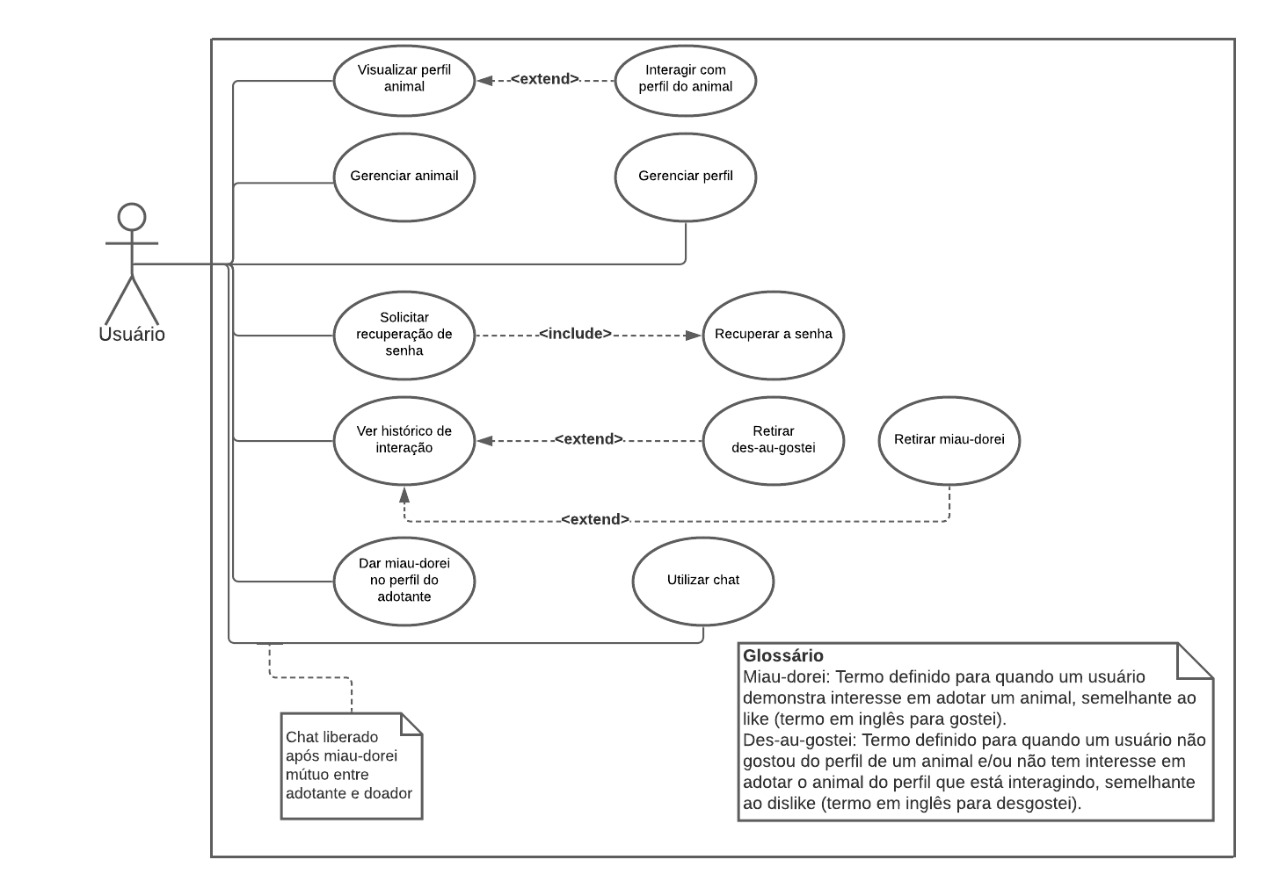
\includegraphics[scale=0.4,angle=90]{imagens/CasosDeUsoPETINDER.jpeg}
	\caption{\label{diagama-casos}Diagrama de Casos de Uso do Sistema}
	\fonte{Elaborada pelos autores}
\end{figure}

\section{Tecnologias utilizadas}
As tecnologias definitivas utilizadas pela equipe no projeto foram determinadas  na \ac{POC}, assim como mostra o \autoref{provaconceitual-pdfpages}.  
\subsection{Para a aplicação}
\ac{HTML}: é uma linguagem de marcação de hipertexto para apresentar e estruturar o conteúdo na \textit{web} \cite{html}.

\ac{CSS}: é uma "folha de estilo" composta por “camadas” e utilizada para definir a apresentação (aparência) em páginas da \textit{internet} que adotam para o seu desenvolvimento linguagens de marcação \cite{css}.

JavaScript: é uma linguagem de programação criada em 1995 por Brendan Eich enquanto trabalhava na Netscape Communications Corporation \cite{jsum}. É uma linguagem de programação de alta complexidade, mas de fácil uso, voltada para criar elementos em aplicações \textit{web}, como sites, aplicativos e sistemas \textit{online} \cite{jsdois}. 
Durante o desenvolvimento foi utilizada uma \ac{API} da tecnologia, denominada "GeoLocation", a qual possibilita acessar a localização do usuário em tempo real.

Bootstrap 5: foi inicialmente criado por Mark Otto e Jacob Thornton para o desenvolvimento web mais rápido e prático. Ele contém todos os tipos de templates baseados em HTML e CSS para várias funções e componentes. Por exemplo: navegação, sistema de grades, carrosséis de imagens e botões. A lista não é exaustiva.  \cite{bootstrap}.

\ac{PHP} é uma linguagem de programação utilizada por programadores e desenvolvedores para construir sites dinâmicos, extensões de integração de aplicações e agilizar no desenvolvimento de um sistema \cite{php}.

CodeIgniter: esse \textit{framework} de desenvolvimento de aplicações, se compararmos com outros, disponibiliza um conjunto de classes que podem ser combinados e estendidos para que aplicações sejam construídas, nos poupando um considerável tempo de codificação \cite{codeigniter}.
Durante o desenvolvimento foram utilizadas bibliotecas do \textit{framework}, como a de envio de e-mail através do protocolo \ac{SMTP}, a de validação de formulários e a de \textit{upload} de imagens. Além disso, também foi utilizada a biblioteca de testes unitários disponível no \gls{CodeIgniter} para realizar os testes automatizados da aplicação, assim como consta no \autoref{testes}.

Visual Studio Code: é um editor de código-fonte leve desenvolvido pela Microsoft. Possui as funcionalidades mais simples como: edição de código com suporte a várias linguagens de programação, terminal de comandos integrado e controle de versão \cite{vscode}.

PostgreSQL: é um \ac{SGBDOR}, desenvolvido como projeto \textit{software} livre, é de código e conta com recursos como: consultas complexas, chaves estrangeiras, integridade transacional, controle de concorrência multi-versão, suporte ao modelo híbrido objeto-relacional, \textit{trigger}, \textit{views} e \textit{stored procedures} em várias linguagens \cite{postgresql}.

PostGIS: é uma extensão geoespacial para o \ac{SGBDOR} \gls{PostgreSQL}. Este módulo é uma robusta solução para o suporte ao armazenamento, gerenciamento, tratamento e análise de dados espaciais \cite{postgis}.

Leaflet: É uma biblioteca JavaScript de código aberto para mapas interativos compatíveis com dispositivos móveis. Pesando apenas cerca de 39 KB de JS, ela tem todos os recursos de mapeamento que a maioria dos desenvolvedores precisa \cite{mapa}.

Azure: É uma plataforma da Microsoft formada por uma série de ferramentas diferentes que libera o acesso a empresas e desenvolvedores, a capacidades de processamento e armazenamento dos \textit{datacenters} da Microsoft. O projeto PETINDER foi hospedado na plataforma Azure. O \ac{IFSP} disponibiliza aos alunos um convênio para assinatura estudantil que fornece créditos que podem ser utilizados na plataforma. A equipe optou por esse serviço de hospedagem pelos seguintes fatores: certificado \ac{SSL} com nota A (\autoref{teste-ssl} e o acesso ao bando de dados \gls{PostgreSQL} e sua extensão geoespacial \gls{PostGIS} \cite{azure}.

\subsection{Requisitadas pela disciplina}
Subversion: é uma ferramenta de controle e versionamento. A equipe utilizou para compartilhar as versões mais recentes da aplicação e da documentação.

\LaTeX:  é um sistema ou programa de marcação para a editoração de documentos de alta qualidade tipográfica, específico para a elaboração de textos científicos. Trata-se de um conjunto de macros ou marcações para o processador de textos TeX \cite{latex}.

YouTube: o site surgiu em virtude do inconveniente que era compartilhar arquivos de vídeo, já que estes eram muito grandes, o que dificultava seu envio por e-mail. O site permite que os usuários coloquem seus próprios vídeos na rede, sendo visualizados por qualquer pessoa no mundo inteiro \cite{youtube}. A equipe utilizou desta tecnologia para postar os vídeos solicitados pela disciplina.

Blogger: é a plataforma gratuita de \textit{blogs} do Google. Além de ser fácil de navegar e administrar, oferece a hospedagem e diversos recursos que permitem ao usuário criar seu \textit{blogs} e personalizá-lo, de acordo com suas necessidades \cite{blogger}. A equipe utilizou desta tecnologia para postar relatórios semanais  solicitados pela disciplina.

%---------------------------------------------
\section{Infraestrutura do banco de dados}
Um banco de dados como o nome nos sugere, é um conjunto de informações coletadas e organizadas de modo que seja usada eficientemente. Um bom exemplo que temos é um livro de receitas, no qual os dados contidos no mesmo são organizados em sua maioria em ordem alfabética, nos auxiliando a achar o que desejamos.

Sabe-se que cada banco de dados, no entanto, possui sua estrutura e particularidade, dessa forma é pertinente que falemos dos meios que são usados para guiar tais estruturas. A começar pelo Modelo de Entidade-Relacionamento (MER), tal modelo analisa determinados acontecimentos na vida real, coleta e realiza um conjunto de elementos básicos organizados em entidades e relacionamentos, a partir desse modelo é possível ter uma pequena noção da estrutura.

Outrossim, faz-se necessário mencionarmos o Diagrama de Entidade-Relacionamento (DER). De forma geral ele é o resultado do que tivemos do Modelo de Entidade-Relacionamento, é menos abstrato e uma maneira de facilitar a visualização do conceito que se tem no \textit{MER}, logo, com ambos os meios pode-se ter uma ideia geral do caminho da estrutura mais completa, na qual o modelo nos traz o conceito do banco de dados e o diagrama nos ajuda a ter uma visão de tal conceito de forma mais organizada e ajustada.

\begin{figure}
    \centering
    \caption{Modelo Entidade Relacionamento}
    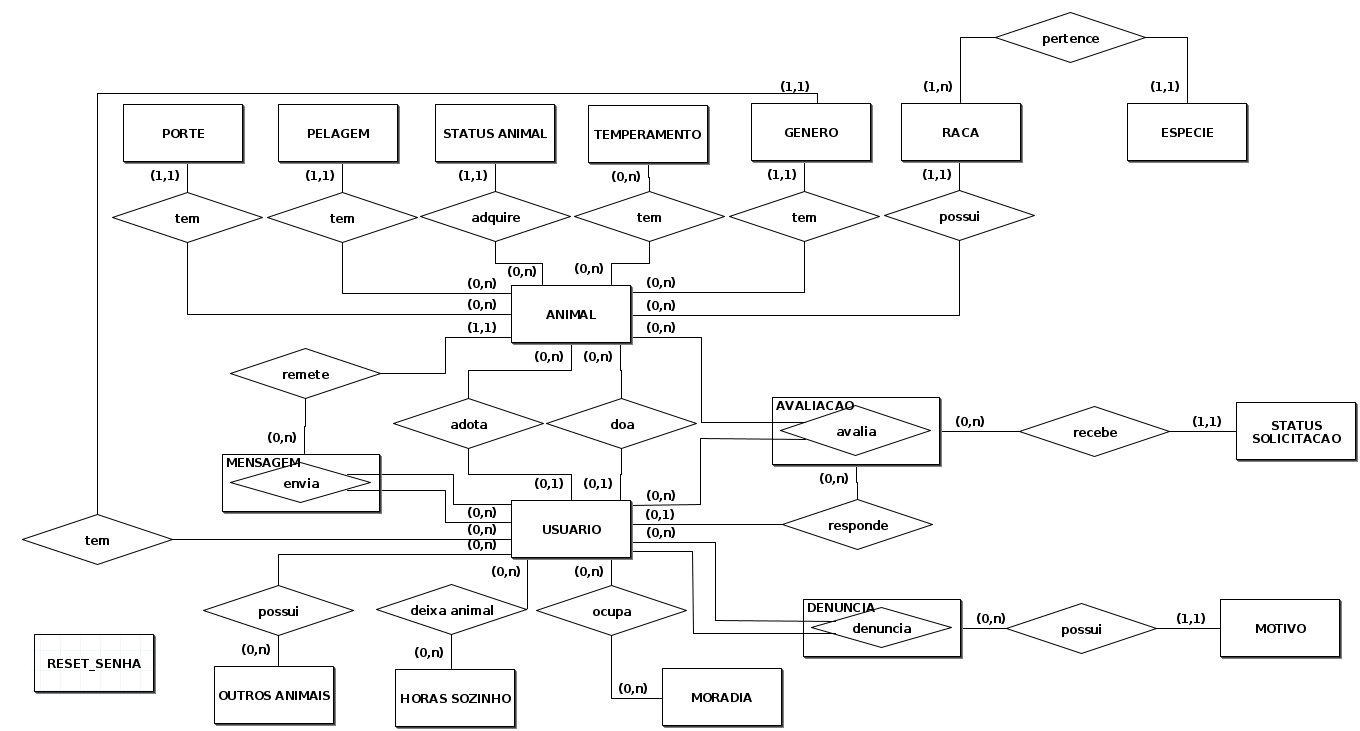
\includegraphics[scale=0.5,angle=90]{imagens/MODELOCONCEITUAL.png}
    \label{mer}
    \fonte{Elaborado pelos autores}
\end{figure}

\begin{figure}
    \centering
    \caption{Modelo Entidade Relacionamento}
    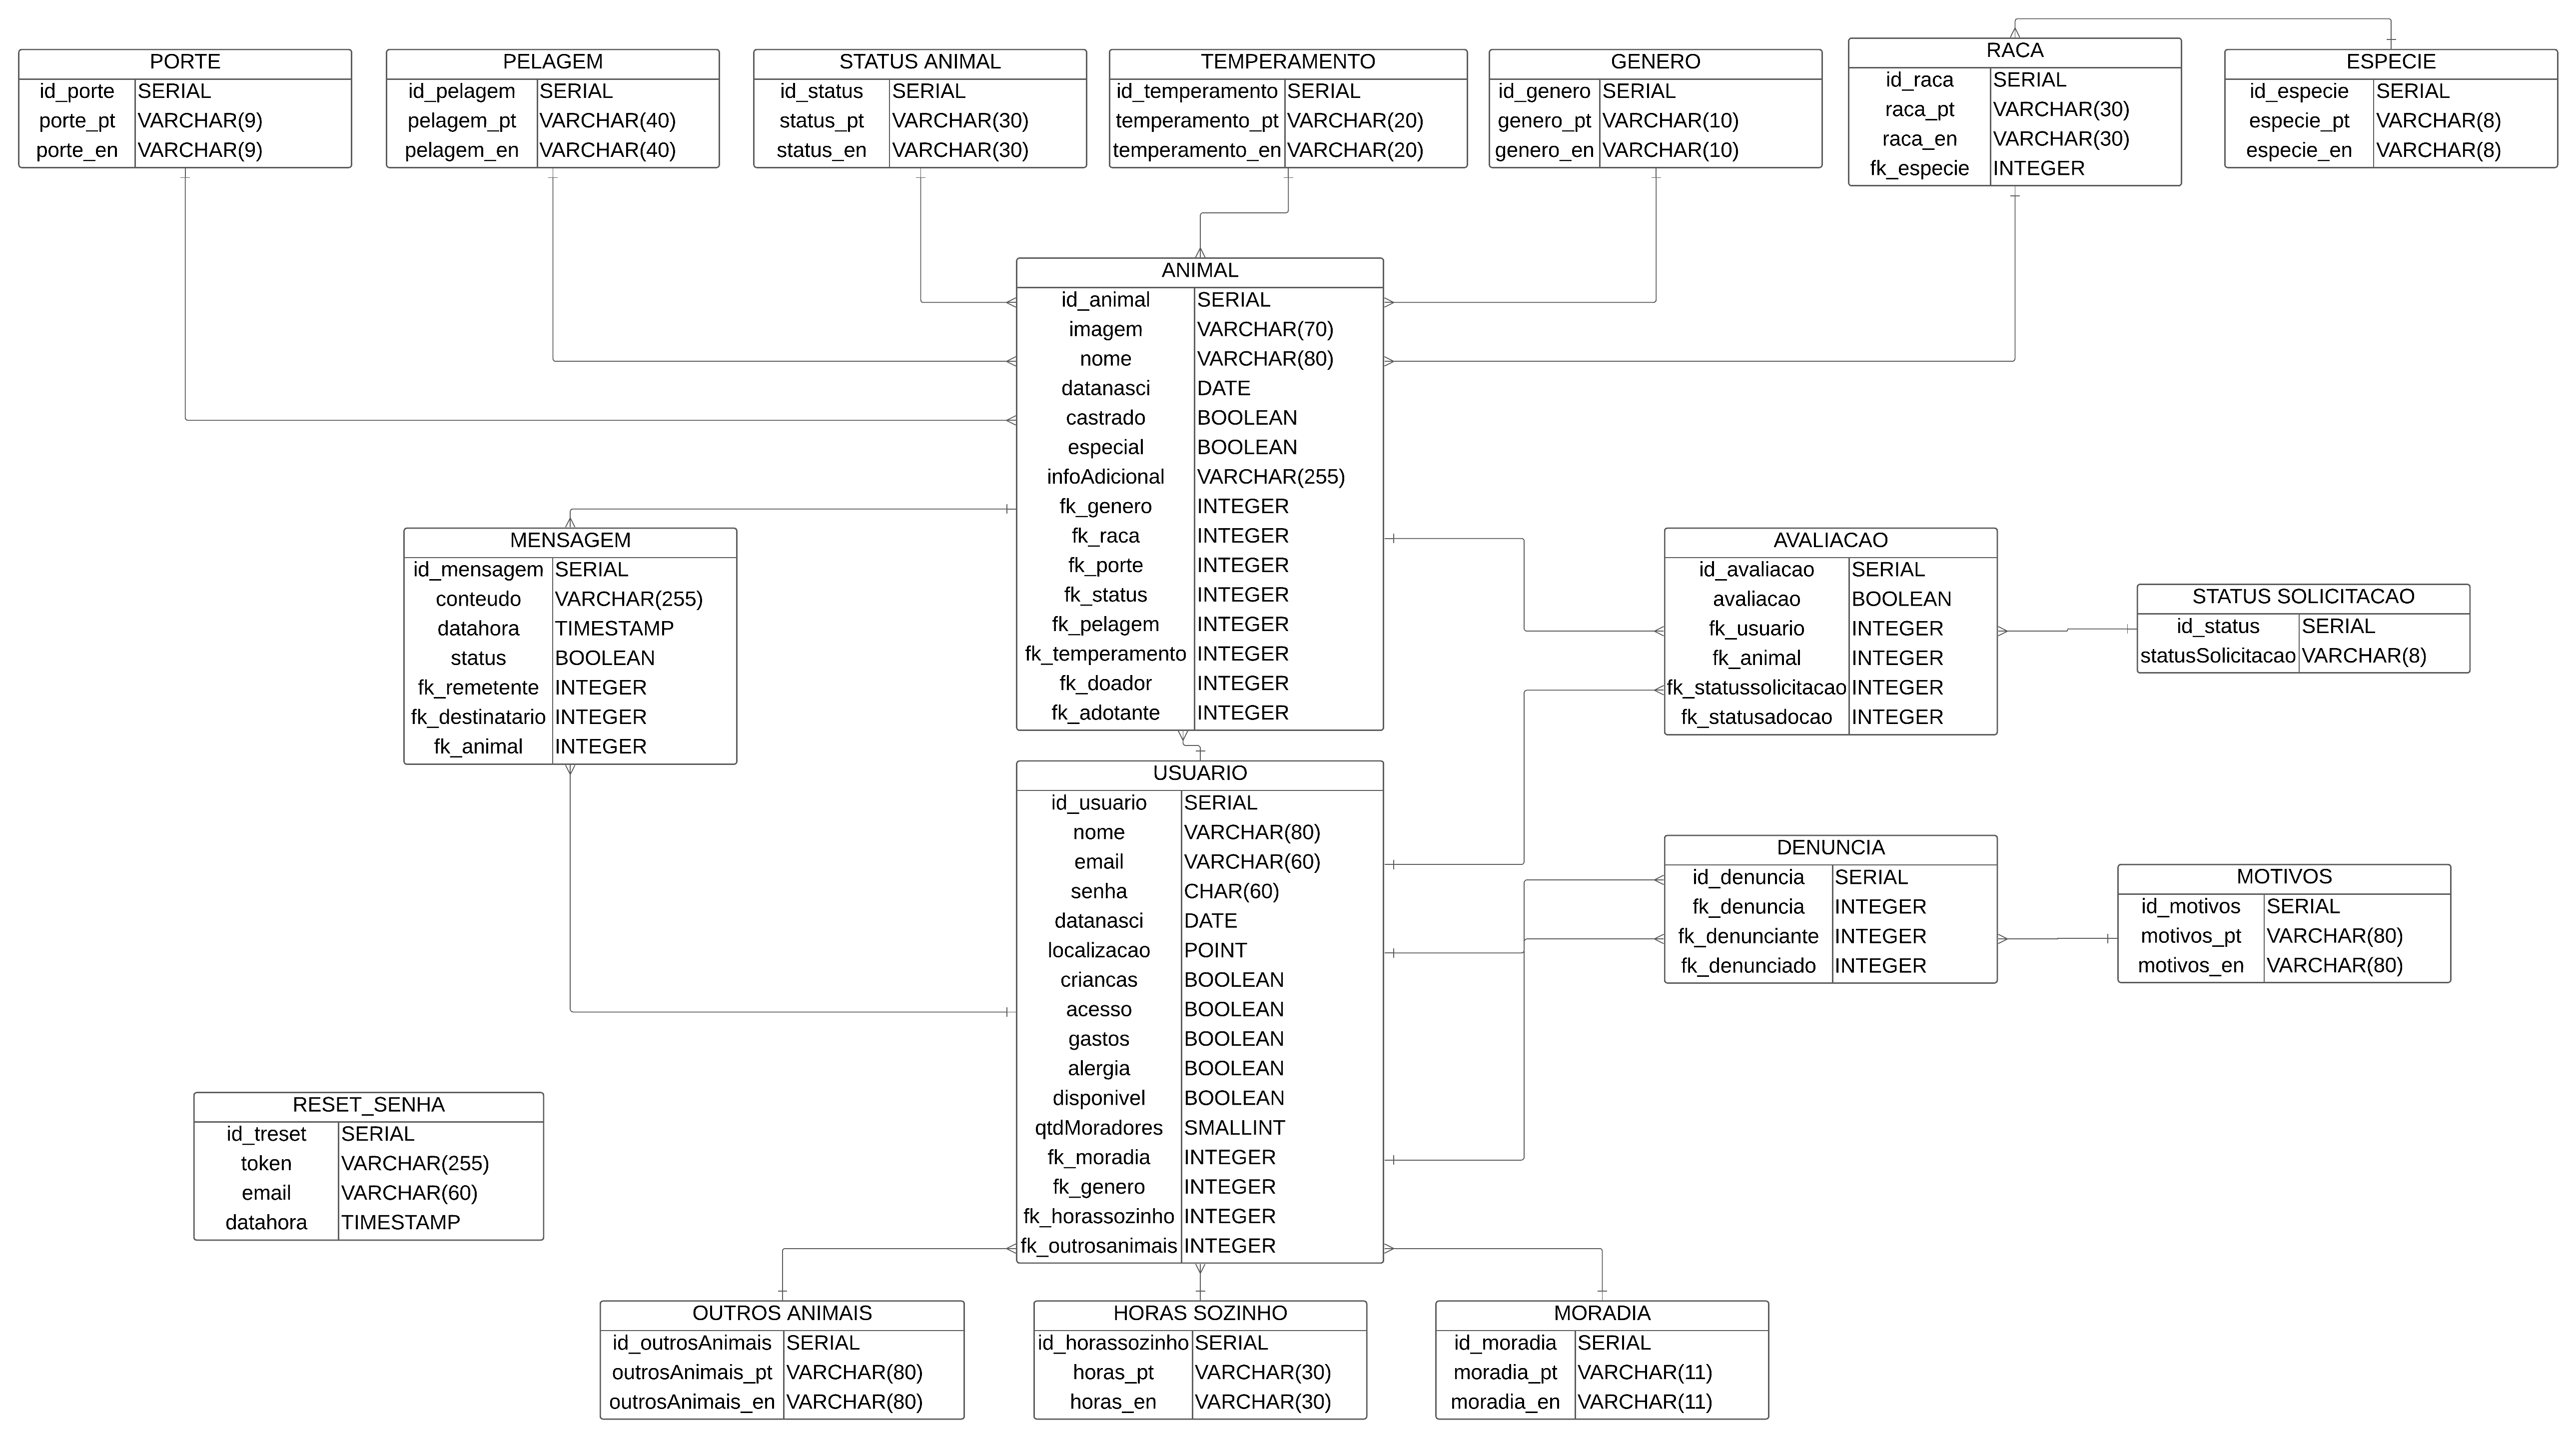
\includegraphics[scale=0.5,angle=90]{imagens/MODELOLOGICO.png}
    \label{der}
    \fonte{Elaborado pelos autores}
\end{figure}

\chapter{Desenvolvimento}
O presente capítulo visa transparecer o processo de desenvolvimento do projeto PETINDER. Tal processo foi registrado em publicações semanais no blog da equipe (\autoref{publicacoes-blog}); em vídeos no canal do \gls{YouTube}, o qual pode ser acessado na (\autoref{qr-url-2}); no repositório que pode ser acessado na \autoref{qr-rep}; e o \textit{site} para acessa-lo, basta usar a (\autoref{qr-url-1}).

\begin{figure}[htb]
\caption{\label{qr-url-1}URL da aplicação}
\begin{pspicture}(25mm,25mm)
\psbarcode{https://petinderapp.azurewebsites.net/}{eclevel=H width=1.0 height=1.0}{qrcode}
\end{pspicture}
\legend{\url{https://petinderapp.azurewebsites.net/}}
\fonte{Elaborado pelos autores}
\end{figure}

\begin{figure}[htb]
\caption{\label{qr-rep}Repositório SVN}
\begin{flushright}
\begin{pspicture}(25mm,25mm)
\psbarcode{https://svn.spo.ifsp.edu.br/svn/a6pgp/A2021-PDS431/TI.TI.TI/}{eclevel=H width=1.0 height=1.0}{qrcode}
\end{pspicture}
\legend{\url{https://svn.spo.ifsp.edu.br/svn/a6pgp/A2021-PDS431/TI.TI.TI/}}
\fonte{Elaborado pelos autores}
\end{flushright}
\end{figure}

\begin{figure}[htb]
\caption{\label{qr-url-2}Canal da equipe no Youtube}
\begin{pspicture}(25mm,25mm)
\psbarcode{https://www.youtube.com/channel/UCbgWTXMmWO9rkkGh8TA2l8Q}{eclevel=H width=1.0 height=1.0}{qrcode}
\end{pspicture}
\legend{\url{https://www.youtube.com/channel/UCbgWTXMmWO9rkkGh8TA2l8Q}}
\fonte{Elaborado pelos autores}
\end{figure}

\begin{figure}[htb]
\caption{\label{qr-blog}Blog da equipe}
\begin{flushright}
\begin{pspicture}(25mm,25mm)
\psbarcode{https://equipetititi.blogspot.com/}{eclevel=H width=1.0 height=1.0}{qrcode}
\end{pspicture}
\legend{\url{https://equipetititi.blogspot.com/}}
\fonte{Elaborado pelos autores}
\end{flushright}
\end{figure}

\section{Ideia inicial}
Como ideia inicial para o projeto, a equipe TI TI TI pensou em um aplicativo de adoção e doação de cães e gatos, em que foi nomeado de PETINDER, em semelhança ao aplicativo de namoro já conhecido, \gls{Tinder}. 

As funcionalidades da ideia inicial seriam:

\begin{itemize}

\item Encontrar animal: processo que possa ser realizado de três maneiras distintas, sendo a primeira de modo manual, onde o usuário procura na listagem de animais registrados no sistema aquele que mais o interesse; a segunda através de filtros, onde, conforme as preferências do usuário, exibe-se uma lista de animais compatíveis com as características estabelecidas pelo usuário no processo de filtragem; e a última, através da "Combinação Perfeita", onde o sistema lista os animais com características compatíveis com as informações fornecidas no formulário de adoção pelo adotante;

\item Delimitar distância: o sistema lista apenas animais que possuam localização próxima ao adotante;

\item \gls{Match}: quando o usuário encontra o animal de sua preferência ele pode curtir o perfil do mesmo. A curtida gera uma notificação para o doador que pode corresponde-la ou não. Caso ele corresponda, o sistema colocará ambos em contato através do \textit{chat} disponível na plataforma, e mudará o status do animal de "disponível" \space para "em processo de adoção". Outros usuários ficarão impossibilitados de curti-lo, porém, poderão ficar em uma fila de espera, caso a adoção não ocorra;

\item Monitorar \textit{chat}: tal funcionalidade proporciona uma restrição de palavras ofensivas, ou seja, caso  o usuário use uma linguagem inapropriada, ele comete uma infração, atingindo o limite de três infrações, este usuário pode ser banido do PETINDER.

\end{itemize}

Por fim, no início do desenvolvimento a equipe optou pelas seguintes tecnologias: 

\begin{itemize}
\item Front-end: \ac{HTML}5, \ac{CSS}3 e \ac{JS};

\item Framework: \gls{Bootstrap} 5;

\item Back-end: \ac{PHP};

\item Banco de dados: \gls{PostgreSQL} com a extensão \gls{PostGIS};

\item IDE: \gls{VSCode} e \gls{Eclipse};

\item Documentos: \gls{Latex};

\item Controle de Versão: \gls{Subversion};

\item \gls{Gource}.
\end{itemize}


\section{Primeiro Bimestre}
No primeiro bimestre (meses maio e junho) houve a criação da equipe TI TI TI e a decisão de dar continuidade no projeto PETINDER, inicialmente desenvolvido pelas integrantes Brenda, Eduarda, Fernanda e Giovana na disciplina técnica \ac{TDS} no ano de 2020.  

A delegação de tarefas deu-se no após a formação da equipe e a escolha do projeto. A equipe realizou reuniões semanais ao longo do projeto através do \gls{Discord} – uma plataforma de comunicação instantânea que permite a troca de mensagens por texto, áudio e vídeo – e utilizaram um grupo no \gls{WhatsApp} para atualizações informais do projeto. 

Quando o projeto PETINDER foi oficialmente aprovado pelos professores da disciplina de \ac{PDS} (\autoref{propostainicial-pdfpages}), a equipe se reuniu para definir a divisão de tarefas de modo que cada integrante contribuísse ao máximo. Nessa reunião foi, também, escolhida como gerente a integrante Giovana Paz. As demais atividades desenvolvidas são mostradas detalhadamente nos Cronogramas Mensais presentes no \autoref{Cronogramas-mensais}.

Nesse bimestre a equipe elaborou a Proposta Inicial, incluída no  \autoref{propostainicial-pdfpages}, dedicando-se à documentação e à apresentação. Foi feito, também, o levantamento das tecnologias a serem utilizadas para o desenvolvimento do \textit{website}.

As tarefas realizadas no primeiro bimestre contaram com a participação integral de todas as integrantes da equipe, assim como mostra os cronogramas mensais através das reuniões semanais realizadas pelo \gls{Discord}. 

\section{Segundo Bimestre}
No segundo bimestre a equipe focou no avanço da aplicação e da documentação para a apresentação da \ac{POC}.
Durante esse bimestre, a equipe definiu o servidor de hospedagem, depois de alguns testes e pesquisas explicados mais detalhadamente em \autoref{mudancas}, que melhor atendia as necessidades do projeto, sendo este o Azure.

Durante o desenvolvimento, ocorreu um problema com o servidor de hospedagem e os créditos estudantis oferecidos pela plataforma para a conta de uma das integrantes da equipe, onde estava alocada a aplicação. Isso porque a configuração padrão do Azure, definida quando criada a aplicação, não era compatível com os serviços oferecidos pela plataforma de forma gratuita para contas de estudantes, assim como as horas de disponibilidade do banco de dados, que, gratuitamente são no máximo 750 horas, e, como a equipe não se atentou a isso, o tempo máximo foi atingido e o serviço ficou indisponível. Devido a isso, o site foi migrado para a conta de outra integrante, onde a aplicação foi criada com as configurações gratuitas da plataforma, e o servidor do banco de dados passou a ser desligado enquanto o site não estivesse sendo usado, ou seja, em manutenções ou apresentações.

Houve a conclusão da comunicação cliente-servidor e banco de dados, do diagrama de arquitetura do sistema, das regras de negócio, requisitos funcionais e não funcionais, também foi gravado e disponibilizado no \gls{YouTube} o vídeo de aderência da \ac{POC}, como solicitado pela matéria.

A equipe concluiu a documentação, encontrada no \autoref{provaconceitual-pdfpages}, e os \textit{slides} para a apresentação da \ac{POC}. Após esta apresentação, a equipe começou a se reorganizar para dar início a documentação final e avançar com a aplicação. Assim, foi iniciado o agrupamento de informações sobre oque era solicitado para a presente documentação e a organização dos apêndices que precisariam ser apresentados.

A realização das tarefas relacionadas à \ac{POC} contaram com a participação integral de todas as integrantes, seja nas reuniões ou na realização das tarefas. Após este momento a integrante Cecília Duarte não participou por mais de 2 semanas das atividades por problemas pessoais, passando a colaborar na realização das tarefas e da presente documentação uma semana antes da apresentação parcial.

\section{Terceiro Bimestre}
Ao decorrer do período de férias entre o primeiro e segundo semestre, estivemos reorganizando as tarefas para o terceiro bimestre, pois, seria necessário acelerar a finalização tanto do documento, quanto do \textit{website}, em preparação para a apresentação final. Após nos reorganizarmos, além de fazer os reajustes que nos foi solicitado, voltamos de fato ao desenvolvimento do projeto em busca de avanços, dos quais serão citados ao longo do capítulo.

Ao decorrer dos desdobramentos do projeto, a nossa equipe aprimorou a função de distâncias em quilometragem adicionando o mapa para facilitar a visualização. Ajustamos o \gls{Miau-dorei} e \gls{Des-au-gostei}, do qual houve implementação do bate-papo, que é aberto após o \gls{Match}, também temos a adoção efetivada, após ocorrer a adoção, é registrado que a mesma ocorreu, para que os adotantes que ainda estão procurando o cão e/ou gato fiquem cientes. Além disso, assim como falado na apresentação do \autoref{propostainicial-pdfpages}, nós adicionamos ao nosso \textit{website} a denúncia, porém, assim como mencionado na \autoref{mudancas}, fizemos algumas alterações, em que, caso o usuário se sentir ameaçado e/ou provocado, aciona essa função, e sendo três denúncias, o usuário que foi denunciado sofre um banimento. Não menos importante, completamos a funcionalidade de combinação perfeita que é explicada no \autoref{propostainicial-pdfpages}.

Por fim, assim como foi sugerido pelos nossos orientadores, acrescentamos a opção de filtro. Sua função principal é que o usuário tenha mais facilidade ao procurar o cão e/ou gato, filtrando as suas preferências, podendo desfazer essa alteração futuramente também. Quanto a documentação, estivemos terminando as tabelas de métricas e o modelo de casos de uso, e finalizamos os textos que precisavam de informações que só poderiam ser obtidas ao fim do projeto. Assim, ao terminar a elaboração da apresentação inicial e ao finalizar o sistema conseguimos concluir a documentação.

\section{Quarto Bimestre}
Após as apresentações de todos os projetos nós desenvolvemos documentos de análise das aplicações de todas as equipes que se apresentaram no terceiro bimestre, contendo uma breve introdução sobre os projetos; pontos que achamos positivos; sugestões de melhoria que consideramos plausíveis; e um resumo sobre suas apresentações. Nós consultamos os documentos que discorriam sobre nossa apresentação e anotamos os pontos de sugestão de melhoria, discutimos a relevância deles em conjunto aos professores orientadores na primeira semana após apresentações.

Em seguida, nossa equipe realizou as alterações sugeridas pelos integrantes da banca na apresentação inicial. Na aplicação, os erros de \ac{PHP} que apareciam durante o funcionamento da interface foram tratados, e foram adicionadas informações sobre a política de adoção, sobre o PETINDER e um vídeo a respeito de adoção de animais na própria plataforma. Nós também adicionamos um botão de direcionamento do usuário a uma página com informações sobre denúncias de maus tratos (como sugerido pela banca) e limitamos o cadastro de animais a usuários que permitam o acesso a sua localização. Por fim, na modelagem de dados do sistema, a tabela responsável por armazenar o \textit{token} correspondente à solicitação de recuperação de senha pelo usuário passou a se relacionar com a tabela de usuários.

Nesse bimestre também foi gerado o documento \gls{Latexdiff}, o qual destaca as diferenças entre as versões do relatório de desenvolvimento entregue pela equipe no bimestre anterior e no atual. Outros requisitos obrigatórios da disciplina que a equipe cumpriu no quarto bimestre foi a gravação e postagem, no nosso canal do \gls{YouTube}, de um vídeo (com duração aproximada de 10 minutos) demonstrando o funcionamento da nossa aplicação após as alterações realizadas no bimestre, e a planilha de notas da equipe.

Ao final do desenvolvimento do projeto foi obtida a \autoref{tab-metricas}, a qual registra as informações de desenvolvimento e apresenta a evolução do PETINDER durante o ano letivo.

\begin{table}[h]
\centering
\ABNTEXfontereduzida
\caption{Métricas}
\label{tab-metricas}
\begin{tabular}{lrrrrrrr}
\hline
\thead{Item} & \thead{Maio} & \thead{Jun} & \thead{Jul} & \thead{Ago} & \thead{Set} & \thead{Out} & \thead{Nov} \\ \hline
Arquivos                                          & 1    & 20     & 32    & 39       &47  &54 &58 \\
Atributos                                         & 0    & 9      & 64    & 77       & 82  &90 &90    \\
Classes                                             & 0    & 1      & 11     & 12      &20 &25 &26   \\
Commits                                      & 2    & 14     & 28  &42       & 43  &46 &49           \\
Dados sobre análises estáticas                    & 0    & 0      & 0   &0       & 1 &1 &1          \\
Entidades de banco de dados & 0    & 8      & 11  &13       &17 &18 &18                                   \\
Imagens                                           & 0    & 0      & 1     & 2       & 2 &2 &2            \\
Interfaces                                        & 0    & 7      & 11     & 10      &22 &25 &30            \\
Linhas                                            & 0    & 610    & 1198    & 2633      &4457 &4602 &4690        \\
Métodos                                           & 0    & 9      & 34     & 43       &117 &125 &129            \\
Postagens do Blog                                 & 2    & 7      & 11   & 16   & 20  &24 & 28             \\
Requisitos                                        & 0    & 18     & 16  & 16       & 16 &16 &14         \\
Reuniões                                          & 4    & 14     & 23   & 24       & 24 &27 &28            \\
Tamanho do Projeto \textit{(MB)}         & 0    & 0 & 2     & 3.6       & 4.3 &6.5 &7.0           \\
Testes                                            & 0    & 1      & 1   & 1       & 3 &4 &4          \\
Testes Unitários/automatizados                  & 0    & 0      & 0   & 0       & 1 &1 &1           \\
Vídeos gerados                                    & 0    & 1      & 3   & 4       & 4 &6 &8        \\ \hline
\end{tabular}
\fonte{Elaborado pelos autores}
\end{table}

\section{Mudanças e descartes}
\label{mudancas}

Durante o desenvolvimento foram necessários alguns ajustes e descartes de ideias, para melhor adequação ao tempo disponível e aos objetivos da equipe. Tais alterações estão detalhadas ao longo desta seção.

O monitoramento do \textit{chat}, foi descartado, seguindo uma sugestão dos professores da disciplina, porque essa funcionalidade precisaria de uma "pré definição" \space de palavras consideradas ofensivas, o que agregaria mais trabalho do que o necessário para o projeto, sobretudo porque essa pré definição poderia trazer problemas futuramente, visto que algumas frases integram algumas das palavras consideradas ofensivas, por isso, essa função poderia acabar punindo um usuário que não tivesse realmente cometido uma infração. Assim, ocorreram ajustes para que esse monitoramento fosse substituído por um sistema de denúncias, no qual, caso um usuário se sinta ameaçado e/ou provocado, ele aciona essa função, e em caso de três denúncias, o infrator seja devidamente banido da plataforma.

Além disso, a equipe optou por usar a tecnologia \gls{CodeIgniter} no desenvolvimento do sistema, pois, além de diminuir o trabalho de fazer inúmeros códigos, facilita na organização deles.

Para o servidor de hospedagem, a escolha inicial foi o \gls{000Webhost}, um servidor gratuito que hospedava o site PETINDER, porém, ele não gerava o certificado \ac{SSL} e não oferecia a segurança \ac{HTTPS}. A segunda opção testada pela equipe foi o \gls{Heroku}, um dos serviços de hospedagem sugeridos pelos professores, sendo uma plataforma gratuita - com a conta de estudantes -  e que oferece a segurança \ac{HTTPS},  entretanto, o certificado \ac{SSL} gerado era nível B. 

Para atender a exigência da disciplina em relação ao certificado de segurança nível A, a equipe migrou para o Azure, uma plataforma em nuvem da empresa Microsoft que fornece um plano gratuito para os estudantes do \ac{IFSP}. 

Também foi considerada a ideia de que as imagens seriam armazenadas no banco através do tipo de dados \ac{BLOB}, entretanto, essa prática não é indicada devido à sobrecarga do banco que o armazenamento de dados tão grandes pode causar. Dessa forma, a equipe decidiu que o armazenamento seria feito em um diretório da aplicação e apenas os nomes das imagens no banco de dados.

Por fim, após a apresentação inicial, foram alterados os termos "\gls{Match} Perfeito" para "Encontrar seu animal", devido à perfeição que o termo sugere não corresponder à funcionalidade, já que esta retorna ao usuário diferentes animais compatíveis com ele, e os termos \gls{Miau-dorei} e \gls{Des-au-gostei} em inglês, para \textit{like} e \textit{ignore} respectivamente, a fins de melhor entendimento por parte dos usuários.

% ---
% Conclusão (outro exemplo de capítulo sem numeração e presente no sumário)
% Dependendo do trabalho desenvolvido ele pode ter uma Conclusão ou Considerações finais
% Para trabalhos de disciplina utilizar Considerações Finais
% ---
\chapter*{Considerações Finais}
